\documentclass[12pt]{article}
\setcounter{section}{-1}
\usepackage{graphicx}
\usepackage[T1]{fontenc}
\usepackage{tikz}
\usepackage{tikz-qtree}
\usepackage{pst-node, pst-asr}
\usepackage{amsmath}
\usepackage{placeins}


\begin{document}

\title{%
 Face and Digit Classification \\
  \large CS440 - Intro to Artificial Intelligence}

\author{Alexander Rozenblit}


\maketitle

\section*{Features}
For every algorithm for both digits and face, I used each pixel as a feature. So, for every digit the feature array was a 2 dimensional 28 by 28 array. For each face the feature array was a 2 dimensional 60 by 70 array. I computed the feature arrays by iterating through the data and putting a 1 in the array if the pixel is a '+' or '\#' and a 0 if the pixel is white space.

\section*{Naive Bayes Classifier}
\section*{Digits}
For the Naive Bayes Classifier for digits I first went through all the training data and added up the features. So I made a 3 dimensional array that was made up of 10, 28 by 28 arrays. Let's say I was traversing a digit that was labeled an "8", I would go to the 8th index of the 3D array, and increment each element if the image had a pixel there. After going through all the training data, and incrementing each element like that, I divided each element of each digit by the frequency of that digit. So, if there were 500 "8"'s I would divide each element in the 8th array by 500. After this process I ended up with a 3D array that showed the probability that there was a pixel in that spot given it was that specific digit . For example if array[0][3][5] had 0.15 in it at that spot. That means that given the digit is a 0 there is a 15\% chance that the spot 3,5 has a pixel in it.\\\\
Using this array I could now apply Bayes rule and start making predictions on the test data. For each test digit, I computed the probability that it is a 0 or 1 or 2 or ... or 9. To compute the probability that a given test digit is 0 for example, you go through each pixel of the test image. If there is a pixel in that spot you multiply by the probability in the array we computed earlier, and if there is no pixel in that spot you multiply by 1 subtracted by that probability. After this process I ended up with an array with the probability that the test data is a 0 or 1 or 2 or ... or 9. Then you select the biggest probability and the digit that corresponds to that probability is the prediction.\\\\
Analysis of Naive Bayes Classifier on Digits:\\\\

\begin{center}
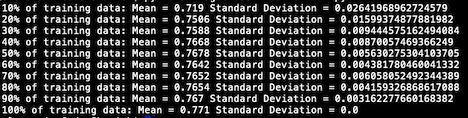
\includegraphics{statsDigBayes.png}
\end{center}

\begin{center}
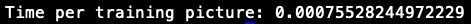
\includegraphics{timeStatsDigBayes.png}
\end{center}

\section*{Faces}
The Naive Bayes Classifier for faces works very similarly to the Naive Bayes Classifier for digits. The only difference is the number of classes. Digits has 10 (one for each digit). Face is binary so only has two classes. So when computing the probabilities only two need to be computed. The two are the probability that the picture is a face and the probability the picture is not a face. The greater probability is picked out of the two and the picture is labeled based on that.\\\\
Analysis of Naive Bayes Classifier on Faces:\\\\

\begin{center}
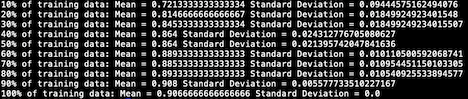
\includegraphics{statsFaceBayes.png}
\end{center}

\begin{center}
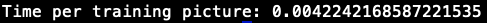
\includegraphics{timeStatsFaceBayes.png}
\end{center}

\section*{Perceptron Classifier}
\section*{Digits}
For the Perceptron Classifier for digits the algorithm works by using a weight vector. Each digit starts with a weight vector that contains 28 * 28 = 784 elements (one for each pixel). The element in the weight vector starts at 0. The algorithm then trains for 10 seconds. It trains by traversing every single image as many times as possible in the given 10 seconds. For each image the algorithm multiplies each pixel by all 10 weight vectors. So for example if a picture has a pixel in spot 0,0, but does not have a pixel in spot 0,1 the program would do $1 * w[0][0] + 0 * w[0][1] + ...$. This process would be repeated for ever spot in the picture and for every weight vector. At the end all the sums are compared and the digit with the greatest sum becomes the prediction. If the prediction is true no weight vectors are changed. However, if the prediction is wrong we do the following: The weight vector of the predicted digit is subtracted by the features of the digit. The weight vector of the true labeled digit is added with the features of the digit. This increases the chances, that if this same image was tested again the program would label it correctly.\\\\
After the 10 seconds of training the weight vectors are used to make predictions on the test images. Each pixel in the image is multiplied by all the weight vectors. The sums are added up just like in the training phase, and the greatest value is picked. The digit corresponding to that value is the prediction.\\\\
Analysis of Perceptron Classifier on Digits:\\\\

\begin{center}
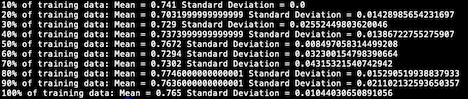
\includegraphics{statsDigPerceptron.png}
\end{center}

\begin{center}
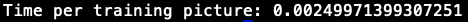
\includegraphics{timeStatsDigPerceptron.png}
\end{center}

\section*{Faces}
The Perceptron Classifier for faces works very similarly to the Perceptron Classifier for digits. The only difference is that the digits algorithm had 10 weight vectors, while the faces one only has two. That is because there are only two classes in the face algorithm: either the picture is a face or it is not. Besides that fact, the algorithms work exactly the same.\\\\
Analysis of Perceptron Classifier on Faces:\\\\

\begin{center}
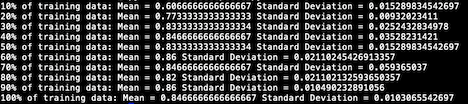
\includegraphics{statsFacePerceptron.png}
\end{center}

\begin{center}
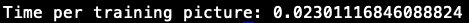
\includegraphics{timeStatsFacePerceptron.png}
\end{center}

\section*{K Nearest Neighbors}
\section*{Digits}
The last algorithm I chose to implement was K Nearest Neighbors. This algorithm works by taking each test image and comparing it with each training image. So for every single test image I computed the euclidean distance between the feature vector of the test image and every single training image. I computed the euclidean distance using the formula for finding the distance between two vectors:\\
\begin{center}
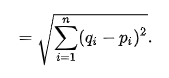
\includegraphics{euclideanDistance.png}
\end{center}
After computing all the euclidean distances, I wanted to find the k smallest distances. I set my k as 5, so for every test image I found the 5 training images that were closest to the test image. Then I looked at the labels for each training image, and the one that occurred most frequently was my prediction for that test image. This process was repeated for every single test image.\\\\
Analysis of K Nearest Neighbors on Digits (Note: Since this algorithm takes multiple hours to run I was only able to run one iteration of it, so that is why the Standard Deviation is 0 throughout).\\\\

\begin{center}
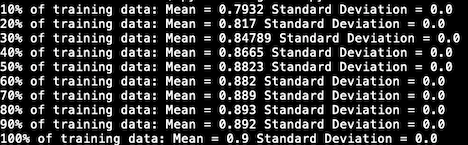
\includegraphics{statsDigKnn.png}
\end{center}

\begin{center}
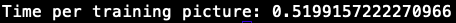
\includegraphics{timeStatsDigKnn.png}
\end{center}

\section*{Faces}
The K Nearest Neighbors algorithm for faces is almost the exact same as the K Nearest Neighbors algorithm for digits. The only difference is that instead of 10 options for a prediction (one for each digit) there are only two.\\\\
Analysis of K Nearest Neighbors (Note: Since this algorithm takes multiple hours to run I was only able to run one iteration of it, so that is why the Standard Deviation is 0 throughout).\\\\

\begin{center}
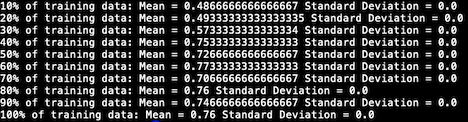
\includegraphics{statsFaceKnn.png}
\end{center}

\begin{center}
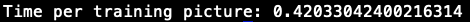
\includegraphics{timeStatsFaceKnn.png}
\end{center}

\section*{Analysis}
\section*{Digits vs. Faces}
For both Naive Bayes Classifier and Perceptron Classifier the algorithms yielded higher accuracy for predicting faces. This makes sense, because in digit prediction the algorithm has to choose between 10 digits, while in face prediction the algorithm only has two choices, this means it is more likely that the algorithms will be able to correctly guess face or not face than a specific digit. \\

\section*{Time}
The most time efficient algorithm was the Naive Bayes Classifier. For the Perceptron Classifier, each training phase was given 10 seconds to run. For this algorithm the time per training picture is irrelevant, because time is independent of the amount of training data the algorithm learns from. The K Nearest Neighbor algorithm was by far the slowest. For digits it took 3 hours and 48 minutes to run one iteration. In comparison with Naive Bayes, K Nearest Neighbors is about 675 time slower.\\

\section*{Accuracy}
Even though the algorithms took varying times to run, the accuracy was generally similar. This is because the same features were used for every single algorithm. For Naive Bayes and Perceptron the accuracy for predicting digits was about 0.77, while the accuracy for predicting faces was near 0.9. This was reversed for the K Nearest Neighbors algorithm where the accuracy for predicting digits was 0.9, and the accuracy for predicting faces was 0.76.\\

\section*{Conclusion}
In conclusion, all these algorithms were able to give good accuracy for both predicting digits and faces. The Naive Bayes Classifier and the Perceptron Classifier make more sense to use, because they are significantly faster, than K Nearest Neighbors and give similar accuracy. 

\end{document}